\chapter{Graph}
    \kactlimport{BFS.java}
    \kactlimport{Tarjan.java}
    \kactlimport{Dikjstra.java}
    \kactlimport{FloydWarshall.java}
    \kactlimport{TopologicalSort.java}
    \kactlimport{MaxFlow.java}
    \kactlimport{StrongConnectedComponents.java}
\section{MaximumBipartiteMatching}
Reducir el problema al de maxflow, crear un nodo source y otro end. Unimos todos los nodos del conjunto 1 a source y del conjunto 2 a end, el flujo maximo que llega a end es la cantidad de aristas escogidas.
\begin{center}
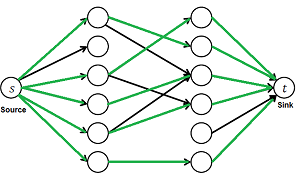
\includegraphics[width=25mm]{content/graph/maximum_matching.png}
\end{center}
